%% bare_conf_compsoc.tex
%% V1.4b
%% 2015/08/26
%% by Michael Shell
%% See:
%% http://www.michaelshell.org/
%% for current contact information.
%%
%% This is a skeleton file demonstrating the use of IEEEtran.cls
%% (requires IEEEtran.cls version 1.8b or later) with an IEEE Computer
%% Society conference paper.
%%
%% Support sites:
%% http://www.michaelshell.org/tex/ieeetran/
%% http://www.ctan.org/pkg/ieeetran
%% and
%% http://www.ieee.org/

%%*************************************************************************
%% Legal Notice:
%% This code is offered as-is without any warranty either expressed or
%% implied; without even the implied warranty of MERCHANTABILITY or
%% FITNESS FOR A PARTICULAR PURPOSE! 
%% User assumes all risk.
%% In no event shall the IEEE or any contributor to this code be liable for
%% any damages or losses, including, but not limited to, incidental,
%% consequential, or any other damages, resulting from the use or misuse
%% of any information contained here.
%%
%% All comments are the opinions of their respective authors and are not
%% necessarily endorsed by the IEEE.
%%
%% This work is distributed under the LaTeX Project Public License (LPPL)
%% ( http://www.latex-project.org/ ) version 1.3, and may be freely used,
%% distributed and modified. A copy of the LPPL, version 1.3, is included
%% in the base LaTeX documentation of all distributions of LaTeX released
%% 2003/12/01 or later.
%% Retain all contribution notices and credits.
%% ** Modified files should be clearly indicated as such, including  **
%% ** renaming them and changing author support contact information. **
%%*************************************************************************


% *** Authors should verify (and, if needed, correct) their LaTeX system  ***
% *** with the testflow diagnostic prior to trusting their LaTeX platform ***
% *** with production work. The IEEE's font choices and paper sizes can   ***
% *** trigger bugs that do not appear when using other class files.       ***                          ***
% The testflow support page is at:
% http://www.michaelshell.org/tex/testflow/



\documentclass[conference,compsoc]{IEEEtran}
% Some/most Computer Society conferences require the compsoc mode option,
% but others may want the standard conference format.
%
% If IEEEtran.cls has not been installed into the LaTeX system files,
% manually specify the path to it like:
% \documentclass[conference,compsoc]{../sty/IEEEtran}





% Some very useful LaTeX packages include:
% (uncomment the ones you want to load)


% *** MISC UTILITY PACKAGES ***

\usepackage{booktabs} % For formal tables
\usepackage{bm}
\usepackage{amsmath}
\usepackage{algorithm}
\usepackage{indentfirst}
\usepackage[noend]{algpseudocode}
\usepackage{multirow}
\usepackage{etoolbox}
\usepackage{siunitx}
\usepackage{graphicx}
%
%\usepackage{ifpdf}
% Heiko Oberdiek's ifpdf.sty is very useful if you need conditional
% compilation based on whether the output is pdf or dvi.
% usage:
% \ifpdf
%   % pdf code
% \else
%   % dvi code
% \fi
% The latest version of ifpdf.sty can be obtained from:
% http://www.ctan.org/pkg/ifpdf
% Also, note that IEEEtran.cls V1.7 and later provides a builtin
% \ifCLASSINFOpdf conditional that works the same way.
% When switching from latex to pdflatex and vice-versa, the compiler may
% have to be run twice to clear warning/error messages.






% *** CITATION PACKAGES ***
%
\ifCLASSOPTIONcompsoc
  % IEEE Computer Society needs nocompress option
  % requires cite.sty v4.0 or later (November 2003)
  \usepackage[nocompress]{cite}
\else
  % normal IEEE
  \usepackage{cite}
\fi
% cite.sty was written by Donald Arseneau
% V1.6 and later of IEEEtran pre-defines the format of the cite.sty package
% \cite{} output to follow that of the IEEE. Loading the cite package will
% result in citation numbers being automatically sorted and properly
% "compressed/ranged". e.g., [1], [9], [2], [7], [5], [6] without using
% cite.sty will become [1], [2], [5]--[7], [9] using cite.sty. cite.sty's
% \cite will automatically add leading space, if needed. Use cite.sty's
% noadjust option (cite.sty V3.8 and later) if you want to turn this off
% such as if a citation ever needs to be enclosed in parenthesis.
% cite.sty is already installed on most LaTeX systems. Be sure and use
% version 5.0 (2009-03-20) and later if using hyperref.sty.
% The latest version can be obtained at:
% http://www.ctan.org/pkg/cite
% The documentation is contained in the cite.sty file itself.
%
% Note that some packages require special options to format as the Computer
% Society requires. In particular, Computer Society  papers do not use
% compressed citation ranges as is done in typical IEEE papers
% (e.g., [1]-[4]). Instead, they list every citation separately in order
% (e.g., [1], [2], [3], [4]). To get the latter we need to load the cite
% package with the nocompress option which is supported by cite.sty v4.0
% and later.





% *** GRAPHICS RELATED PACKAGES ***
%
\ifCLASSINFOpdf
  % \usepackage[pdftex]{graphicx}
  % declare the path(s) where your graphic files are
  % \graphicspath{{../pdf/}{../jpeg/}}
  % and their extensions so you won't have to specify these with
  % every instance of \includegraphics
  % \DeclareGraphicsExtensions{.pdf,.jpeg,.png}
\else
  % or other class option (dvipsone, dvipdf, if not using dvips). graphicx
  % will default to the driver specified in the system graphics.cfg if no
  % driver is specified.
  % \usepackage[dvips]{graphicx}
  % declare the path(s) where your graphic files are
  % \graphicspath{{../eps/}}
  % and their extensions so you won't have to specify these with
  % every instance of \includegraphics
  % \DeclareGraphicsExtensions{.eps}
\fi
% graphicx was written by David Carlisle and Sebastian Rahtz. It is
% required if you want graphics, photos, etc. graphicx.sty is already
% installed on most LaTeX systems. The latest version and documentation
% can be obtained at: 
% http://www.ctan.org/pkg/graphicx
% Another good source of documentation is "Using Imported Graphics in
% LaTeX2e" by Keith Reckdahl which can be found at:
% http://www.ctan.org/pkg/epslatex
%
% latex, and pdflatex in dvi mode, support graphics in encapsulated
% postscript (.eps) format. pdflatex in pdf mode supports graphics
% in .pdf, .jpeg, .png and .mps (metapost) formats. Users should ensure
% that all non-photo figures use a vector format (.eps, .pdf, .mps) and
% not a bitmapped formats (.jpeg, .png). The IEEE frowns on bitmapped formats
% which can result in "jaggedy"/blurry rendering of lines and letters as
% well as large increases in file sizes.
%
% You can find documentation about the pdfTeX application at:
% http://www.tug.org/applications/pdftex





% *** MATH PACKAGES ***
%
%\usepackage{amsmath}
% A popular package from the American Mathematical Society that provides
% many useful and powerful commands for dealing with mathematics.
%
% Note that the amsmath package sets \interdisplaylinepenalty to 10000
% thus preventing page breaks from occurring within multiline equations. Use:
%\interdisplaylinepenalty=2500
% after loading amsmath to restore such page breaks as IEEEtran.cls normally
% does. amsmath.sty is already installed on most LaTeX systems. The latest
% version and documentation can be obtained at:
% http://www.ctan.org/pkg/amsmath





% *** SPECIALIZED LIST PACKAGES ***
%
%\usepackage{algorithmic}
% algorithmic.sty was written by Peter Williams and Rogerio Brito.
% This package provides an algorithmic environment fo describing algorithms.
% You can use the algorithmic environment in-text or within a figure
% environment to provide for a floating algorithm. Do NOT use the algorithm
% floating environment provided by algorithm.sty (by the same authors) or
% algorithm2e.sty (by Christophe Fiorio) as the IEEE does not use dedicated
% algorithm float types and packages that provide these will not provide
% correct IEEE style captions. The latest version and documentation of
% algorithmic.sty can be obtained at:
% http://www.ctan.org/pkg/algorithms
% Also of interest may be the (relatively newer and more customizable)
% algorithmicx.sty package by Szasz Janos:
% http://www.ctan.org/pkg/algorithmicx




% *** ALIGNMENT PACKAGES ***
%
%\usepackage{array}
% Frank Mittelbach's and David Carlisle's array.sty patches and improves
% the standard LaTeX2e array and tabular environments to provide better
% appearance and additional user controls. As the default LaTeX2e table
% generation code is lacking to the point of almost being broken with
% respect to the quality of the end results, all users are strongly
% advised to use an enhanced (at the very least that provided by array.sty)
% set of table tools. array.sty is already installed on most systems. The
% latest version and documentation can be obtained at:
% http://www.ctan.org/pkg/array


% IEEEtran contains the IEEEeqnarray family of commands that can be used to
% generate multiline equations as well as matrices, tables, etc., of high
% quality.




% *** SUBFIGURE PACKAGES ***
%\ifCLASSOPTIONcompsoc
%  \usepackage[caption=false,font=footnotesize,labelfont=sf,textfont=sf]{subfig}
%\else
%  \usepackage[caption=false,font=footnotesize]{subfig}
%\fi
% subfig.sty, written by Steven Douglas Cochran, is the modern replacement
% for subfigure.sty, the latter of which is no longer maintained and is
% incompatible with some LaTeX packages including fixltx2e. However,
% subfig.sty requires and automatically loads Axel Sommerfeldt's caption.sty
% which will override IEEEtran.cls' handling of captions and this will result
% in non-IEEE style figure/table captions. To prevent this problem, be sure
% and invoke subfig.sty's "caption=false" package option (available since
% subfig.sty version 1.3, 2005/06/28) as this is will preserve IEEEtran.cls
% handling of captions.
% Note that the Computer Society format requires a sans serif font rather
% than the serif font used in traditional IEEE formatting and thus the need
% to invoke different subfig.sty package options depending on whether
% compsoc mode has been enabled.
%
% The latest version and documentation of subfig.sty can be obtained at:
% http://www.ctan.org/pkg/subfig




% *** FLOAT PACKAGES ***
%
%\usepackage{fixltx2e}
% fixltx2e, the successor to the earlier fix2col.sty, was written by
% Frank Mittelbach and David Carlisle. This package corrects a few problems
% in the LaTeX2e kernel, the most notable of which is that in current
% LaTeX2e releases, the ordering of single and double column floats is not
% guaranteed to be preserved. Thus, an unpatched LaTeX2e can allow a
% single column figure to be placed prior to an earlier double column
% figure.
% Be aware that LaTeX2e kernels dated 2015 and later have fixltx2e.sty's
% corrections already built into the system in which case a warning will
% be issued if an attempt is made to load fixltx2e.sty as it is no longer
% needed.
% The latest version and documentation can be found at:
% http://www.ctan.org/pkg/fixltx2e


%\usepackage{stfloats}
% stfloats.sty was written by Sigitas Tolusis. This package gives LaTeX2e
% the ability to do double column floats at the bottom of the page as well
% as the top. (e.g., "\begin{figure*}[!b]" is not normally possible in
% LaTeX2e). It also provides a command:
%\fnbelowfloat
% to enable the placement of footnotes below bottom floats (the standard
% LaTeX2e kernel puts them above bottom floats). This is an invasive package
% which rewrites many portions of the LaTeX2e float routines. It may not work
% with other packages that modify the LaTeX2e float routines. The latest
% version and documentation can be obtained at:
% http://www.ctan.org/pkg/stfloats
% Do not use the stfloats baselinefloat ability as the IEEE does not allow
% \baselineskip to stretch. Authors submitting work to the IEEE should note
% that the IEEE rarely uses double column equations and that authors should try
% to avoid such use. Do not be tempted to use the cuted.sty or midfloat.sty
% packages (also by Sigitas Tolusis) as the IEEE does not format its papers in
% such ways.
% Do not attempt to use stfloats with fixltx2e as they are incompatible.
% Instead, use Morten Hogholm'a dblfloatfix which combines the features
% of both fixltx2e and stfloats:
%
% \usepackage{dblfloatfix}
% The latest version can be found at:
% http://www.ctan.org/pkg/dblfloatfix




% *** PDF, URL AND HYPERLINK PACKAGES ***
%
%\usepackage{url}
% url.sty was written by Donald Arseneau. It provides better support for
% handling and breaking URLs. url.sty is already installed on most LaTeX
% systems. The latest version and documentation can be obtained at:
% http://www.ctan.org/pkg/url
% Basically, \url{my_url_here}.




% *** Do not adjust lengths that control margins, column widths, etc. ***
% *** Do not use packages that alter fonts (such as pslatex).         ***
% There should be no need to do such things with IEEEtran.cls V1.6 and later.
% (Unless specifically asked to do so by the journal or conference you plan
% to submit to, of course. )


% correct bad hyphenation here
\hyphenation{op-tical net-works semi-conduc-tor}


\begin{document}
%
% paper title
% Titles are generally capitalized except for words such as a, an, and, as,
% at, but, by, for, in, nor, of, on, or, the, to and up, which are usually
% not capitalized unless they are the first or last word of the title.
% Linebreaks \\ can be used within to get better formatting as desired.
% Do not put math or special symbols in the title.
\title{Efficient Multistream Regression}


% author names and affiliations
% use a multiple column layout for up to three different
% affiliations
\author{Anonymous Authors}

% conference papers do not typically use \thanks and this command
% is locked out in conference mode. If really needed, such as for
% the acknowledgment of grants, issue a \IEEEoverridecommandlockouts
% after \documentclass

% for over three affiliations, or if they all won't fit within the width
% of the page (and note that there is less available width in this regard for
% compsoc conferences compared to traditional conferences), use this
% alternative format:
% 
%\author{\IEEEauthorblockN{Michael Shell\IEEEauthorrefmark{1},
%Homer Simpson\IEEEauthorrefmark{2},
%James Kirk\IEEEauthorrefmark{3}, 
%Montgomery Scott\IEEEauthorrefmark{3} and
%Eldon Tyrell\IEEEauthorrefmark{4}}
%\IEEEauthorblockA{\IEEEauthorrefmark{1}School of Electrical and Computer Engineering\\
%Georgia Institute of Technology,
%Atlanta, Georgia 30332--0250\\ Email: see http://www.michaelshell.org/contact.html}
%\IEEEauthorblockA{\IEEEauthorrefmark{2}Twentieth Century Fox, Springfield, USA\\
%Email: homer@thesimpsons.com}
%\IEEEauthorblockA{\IEEEauthorrefmark{3}Starfleet Academy, San Francisco, California 96678-2391\\
%Telephone: (800) 555--1212, Fax: (888) 555--1212}
%\IEEEauthorblockA{\IEEEauthorrefmark{4}Tyrell Inc., 123 Replicant Street, Los Angeles, California 90210--4321}}




% use for special paper notices
%\IEEEspecialpapernotice{(Invited Paper)}




% make the title area
\maketitle

% As a general rule, do not put math, special symbols or citations
% in the abstract
\begin{abstract}
In the data stream regression problem, the predicted values of data instances are generated from a non-stationary process. According to past studies, scholars were focusing on problems under different scenarios such as covariant shift or concept drift. However, lots of these theories are discussing one scenario while keeping others consistent. For example, the training and testing data distribution are assumed to be similar, and true output value related to stream instances would be available. However, in practice these assumptions are not always valid. For most of the stream regression problems, only a fraction of values may be available soon after the prediction. If we only use a small fraction of data to train the model, sampling bias, or shift of the input distribution may be introduced accordingly. Thus the prediction generated by this data sample would not be accurate, so how to appropriately handling this issue is a challenge for recent work. Moreover, if the conditional probability between the training data sample and testing data sample is different under the data stream setting, more estimation biases will be introduced as well. 

In this paper, we present a setting of multistream regression problem, involving two independent non-stationary data generating process. A source stream continuously generates data instances with values of output while the target stream generates data instances without values of output. Notice here the distribution of instances may vary. Hence the issue we want to address here, which is called Multistream Regression, is to estimate the output of each instance in target stream, while using output available on the source stream. Since the concept drift may occur between these two streams, a concept drift detection framework is designed and implemented. An assemble model is built to update the model built before the concept drift point in the source stream. We empirically evaluate the multistream regression's performance on real-world datasets and artificially generated datasets with synthetic biases.
\end{abstract}

% no keywords




% For peer review papers, you can put extra information on the cover
% page as needed:
% \ifCLASSOPTIONpeerreview
% \begin{center} \bfseries EDICS Category: 3-BBND \end{center}
% \fi
%
% For peerreview papers, this IEEEtran command inserts a page break and
% creates the second title. It will be ignored for other modes.
\IEEEpeerreviewmaketitle

\section{Introduction}
\label{introduction}

Recent  proliferation  of  Internet  technology  in daily life  has been creating numerous stream  data. These data 
streams may comes from  a
variety of sources, such as social networks, online businesses, sensors, military surveillance and so on. Data streams exhibit dynamic characteristics as opposed to static data (e.g. a data warehouse). Hence, unlike traditional datasets, the stream of data flows into a computer system continuously with varying 
arrival rates. They are time stamped, fast changing, massive, 
and potentially infinite. Therefore, traditional database technology has limited capability to store and process an entire data stream due to its tremendous volume. 
Relative mining or analysis algorithms must process the data in real time and update the parameters as the 
stream progresses. 

Regression analysis is a widely  used technique for modeling the relationship between dependent 
variables and independent variables\cite{Friedman}. Several recent approaches focus on applying regression analysis techniques to model and predict the behavior of the 
stream data. Traditionally, the main task of regression is to learn a function with the input of several attributes from the past stream data, and predicting the value of a numerical target attribute in the future stream data \cite{Gama}, \cite{Lughofer}. It is commonly assumed that using the source data with output available to train the linear regression model (pairs of input vectors and output scalars) are representative of the target data. Specifically, in real world, non-stationary  data generation process may 
induce arbitrary changes in data distribution over time. In the past time, series of studies  have  proposed 
techniques to address these challenges. 
% In the  
% Gama\cite{Gama_drift} 's research, he proposed (); and 
Bifet\cite{bifet2007} proposed sliding windows to address the 
shift problem, the window size could be recomputed online according to the rate of change observed from the data in the 
window itself. However, these techniques make  two strong  assumptions on the ability of applications that deploying them. One of the assumptions is that true output value of data instances along the stream will be available soon after 
prediction. The other assumption is that  sample  data distribution of the training and test mini-batches are equal during regression, this assumption may often be violated in many real-world applications. 
Also, in real world, continuous output value are normally obtained using mechanisms such as sensors
under most of the situations, so it may not occur at a fast enough speed. In this case, a sampling data instances  for  prediction  may  be  biased, this  induces  a  difference  in  data  distribution  between  the  training  and test data \cite{braams:babel,clark:pct,herlihy:methodology}.  A regression model trained on such a biased training dataset may perform poorly on future unbiased test data. This is known as data shift \cite{Gama_drift}.

Except data shift, there is another challenge called concept drift\cite{Parker}, which  occurs  in  a  stream  when  the  underlying concept of data changes over time. So, the  regression model needs  to  be  updated  regularly to adapt  to  the  most  recent concept. The  vast  majority  of  concept  drift  researches assume  that  true  output values  of  test instances  will  be  readily  available  to  update  the  regression  as 
soon  as  they  are  tested.  However,  typical  feedback 
are collected from sensors and validated by the human expert, which  is  a  costly  and  time consuming process. More often, true values are available only for a limited amount of data. Therefore, their  assumption suffer in this scenario.

There are very few effective methods that address regression algorithm under the data shift environment. At first, researchers use re-weight method to solve previous problem, but this method introduces strong inductive biases that are highly extrapolative. Recently, a more improved method is proposed in the paper\cite{chen,herlihy:methodology,Fear05}. In this approach, the authors
% citecomm
established a robust bias-aware regression to solve the covariate shift problem that embraces the resulting uncertainty. Their approach assumes that the stochastic mapping from inputs to the output variable is as similar as possible to a ``zero-knowledge'' reference distribution. Then, they apply minimax relative log-loss optimization approach for minimizing relative loss and conditional Kullback-Leibler divergence in the worst case. This approach performs best compared to a range of existing regression models on both synthetic and natural biased datasets. However, it does not consider occurrence of concept drifts. Furthermore, the approach proposed in~\cite{chen,herlihy:methodology,Fear05} does not consider covariate shift between streams generating labeled training data and unlabeled test data.
  
  In  this  paper,  we  introduce  a  new  problem  setting  consisting of different types of data streams over the same domain, thereby relaxing the above-mentioned assumptions. This approach is motivated by MSC algorithm \cite{chandra2016}. We assume the existence of two streams. One stream is referred to as the source stream. This stream consists of data instances, generated by a non-stationary process from a particular domain. Another  stream  of  data  instances from the same domain is assumed to be generated by an independent non-stationary process, referred to as target stream. The regression problem is to predict value of data instances in  the concept  drifting target stream  while  leveraging  real  information  available  in  the  concept  drifting source stream. Since this regression problem involves two types of  data  streams. For example, source  stream with real value and target stream without value, we call it as Multi-Stream Regression. This setting could be illustrated in Figure 1.  
  
  The multistream problem proposed resonates with that of domain adaptation\cite{Ben-David} and transfer learning\cite{Pan} when considering a set of observations in each stream within a particular time window. Here, the training and test distributions are assumed to have equal conditional class distribution  with  unequal  marginal distribution. In this situation under the multistream regression environment, we apply a correction mechanism to weigh training data instances so that their weighted data distribution resembles that of the observed test data distribution. Here are major contributions of this paper:
  
  1. We introduce a new data stream regression setting consisting of two independent non-stationary streams. Output value are predicted in target stream using the data instances from source stream. 
  
  2. We adapt a Robust Covariate-Shift-aware Regression (RCSR) to address challenges in adapting the source data stream distribution, which may be biased, towards the target data stream distribution in a non-stationary environment. 
  
  3. We perform concept drift detection without requiring true dependent variable from the target stream, using dependent variable observed on the source stream. 
  
  4. We evaluate this proposed approach empirically over several benchmark datasets, and compare the results with baseline methods. One baseline method, RCSR, is from the paper\cite{chen}. The other baseline method pRCSR is periodically update model by using RCSR. Our method Efficient Multi-stream Regression (EMR) significantly improved performance of baseline methods.
  
  The rest of the paper is organized as follows: Section 2 discusses the related work and Section 3 provides a background on multiple stream regression. Section 4 then describes the proposed approach, and Section 5 reports the experiments and results. Finally, Section 6 concludes with directions to future work.

\section{Related Work}
\label{notations}
In this section, we present a brief discussion on covariate shift adaptation, concept drift and multistream regression along with some of the related work in this area.

\subsection{Covariate Shift Adaptation}
\label{notations}
One of the fundamental ideas of data mining technology is that both the training and test data 
represent the same data distribution, known as the "stationary
distribution assumption". In the previous statement, we described that this assumption may violates in real-world application. Addressing an arbitrary difference between training and test distribution is a very difficult problem\cite{Huang}. Hence, most approaches assume that the source and target data distributions $P_{src}$ and $P_{tgt}$ are related through a covariate shift assumption. As previous describe, the relationship between the source and target data distributions is such that $P_{src}(y \vert {\textbf{x}}) = P_{tgt}(y \vert {\textbf{x}})$ and $P_{src}(\textbf{x}) \ne P_{tgt}(\textbf{x})$, where x and y denote the
set of covariate values and target value of the data instance respectively.

Recent studies focus on developing correction mechanisms for covariate shift, one algorithm called Kernel Mean Matching (KMM) is proposed in paper [13]. In their algorithm, 
covariate shift between training and test data distribution is accounted by 
computing an importance weight $\beta(\textit{\textbf{x}}) = \frac{P_{tgt}({\textbf{x}})}
{P_{src}({\textbf{x}})}$. For each source instance x, we could use this algorithm in the learning process. Except KMM algorithm, KLIEP\cite{sugiyama}, and unconstrained Least Square Importance Fitting (uLSIF)\cite{kanamori}, are among the available techniques  in the literature for handling covariate shift in data. However, these 
approaches work only for fixed-size training and test data. For stream data, Kawahara 
and Sugiyama\cite{kawahara} extended previous KLIEP to direct online density ratio 
estimation and get good result. But it works on a single stream of data, where set 
of source/reference and target data instances are determined by a sliding window. In 
this paper, we consider multiple streams of data, where new data instance may arrive 
arbitrarily in any stream.


\subsection{Concept Drift}
\label{notations}
  Concept drift refers to the scenario when the relation between input data $X$, feature values, and the target variable $y$ will be changed over time. Formally, concept drift between time $t_0$ and $t_1$ can be defined as

\begin{equation}
   \exists X: P_{t_{0}}(X,{y}) \ne P_{t_{1}}(X,{y})
\end{equation} 

Where $P_{t_{0}}(X,{y})$ represents the joint distribution of the set of input variables $X$ and the target value $y$ at time $t_{0}$, and $P_{t_{1}}(X,{y})$ is the joint distribution at time $t_{1}$\cite{gama_survey}.The  
components of this equation include the prior probability of the target variable
$P_{y}$, the conditional probability $P(X \vert {y})$, distribution of incoming data $P_{X}$, and  the  posterior  probability $P(y \vert 
{\textbf{x}})$. Real concept drift refers  to  the  changes  in  posterior  probability $P(y \vert {\textbf{x}})$. It may occur due to several reasons including changes  in  incoming  data distribution $P_{X}$.
  
  

\subsection{Stream Regression}
Many methods can be found in the literature for solving classification tasks on streams, while only few exists for regression tasks. Especially, there are limited number of paper talking about regression under stream setting with concept drift. An incremental algorithm that scales linearly with the number of examples is presented to solve an incremental model tree problem \cite{Friedman}. The authors present an incremental node splitting rule, together with incremental methods for stopping the growth of the tree and pruning.

Multiple Linear Regression (MLR) analysis is also discussed for time series data stream. It is based on the OLAP technology  for streaming data. This system enables an online computation of linear regression over multiple dimensions, and tracks the change of trend according to user's interest. However, none of the researches mentioned above takes sudden, unusual change of the conditional probability distribution, known as concept drift, in to consideration. Specifically, if we have a multistream setting with concept drift, none of these methods described can learn the change in hidden variables or in the intrinsic properties of the observed variables. Hence the study of this problem is very important.




\section{Preliminaries}

In this section, we formalize the multistream regression problem and present challenges of performing  regression over drifting data streams in this context

\subsection{Multiple Stream Regression}
\label{statement}

Data stream regression is a challenging task due to its  inherent properties, like infinite length, concept drift. Infinite length problem is addressed by dividing 
the whole stream into fixed-size mini-batches. However, previous  work suggesting for regression  data stream are typically based on a single data stream. Recently, multiple data streams model (MDS) and some related issues are discussed in several papers. Although research on multiple data streams model is not started for a long time, multiple  data  streams  has been involved  in  many of the data stream applications, today such as advances in micro-electro-mechanical system, wireless  communication technology and so on.

  From  the  above introduction,  multiple data streams model is  different  from that  single stream model in the following aspects \cite{bowman:reasoning}.The first aspect is multiple data streams model adopts multiple data domain 
% citecom
to generate distributed data streams independently. What's more, there are requirements over all  the  data  streams  such as comparing local  pattern and regional/global  pattern,  and synchronizing data points  from  these  data  streams. Finally, it  is difficult  or  impractical  to  simply  view  and  treat  the  data  from different  data  sources  as  a  single  data  stream  with  multiple marginal probability, which means that source and target data 
represent the same data distribution.
  
  Here, we propose a new problem setting called Multi-stream Regression, in this situation, two data streams over the same domain are considered relaxing the following assumptions:  first, true values of data instances along the stream are not available soon after prediction. Second, with previous statement, source and target data represent different distribution.
  

\begin{table}[H]
\centering
\caption{Notations}
\label{tab1}
\begin{tabular}{|l|l|}
\hline
 Symbol & Meaning \\ \hline
 $D$ & Domain \\ \hline
 $x$ & Independent variables of $m$ dimensions \\ \hline
 $y$ & Value of a data instance \\ \hline
 $S$ & Source data stream with actual $y$ \\ \hline
 $T$ & Target data stream without actual $y$  \\ \hline
 $M$ & Parameter matrix of regression model  \\ \hline
 $\theta$ & Vectorized \\ \hline
 $f_{src}$ & Probability distribution function of source data \\ \hline 
 $f_{tgt}$ & Probability distribution function of target data \\ \hline
 $f_{tm}$ & Probability distribution of target mini batch \\ \hline
 $\hat{Y}$ & Predicted value of a data instance \\ \hline
 $N_{max}$ & Maximum allowable size for dynamic window \\ \hline
\end{tabular}
\end{table}

\subsection{Notations and Problem Statement }
\label{notations}
In this paper, notations listed in Table \ref{tab1} are used to describe concepts of the data stream. 
A continuous stream of 
data instances is generated from domain $D$. A data instance is
denoted as $(x, y)$, where $x$ is a m-dimensional vector, and $y$ is the corresponding value. Two processes $S$ and $T$ in
domain $D$ are used to represent the source and target data stream.
In process $S$, values of both $x$ and $y$ are available, while
in process $T$, only $x$ is available. Thus, a 
$Multi-stream Regression$ problem can be defined as follows:

Suppose $X_{s}$ is a set of n-dimensional vectors and $Y_{s}$ is the corresponding true value  in a certain domain $D$. Meanwhile, $X_{t}$ is a set of 
n-dimensional vectors in a target data stream in the
same domain. We want to build a regression model $f_{ens}$ to
estimate the value that corresponds $X_{t}$ using $X_{s}$,
$Y_{s}$ and $X_{t}$.

\subsection{Challenges}
\label{challenges}
Normally we assume that inputs in the source set follow the
same distribution as the inputs in the target set, so that
source
data provides solid information in predicting instances in
the target set. However, this assumption is not always valid in 
a multistream setting. Equivalently, consider sample
probability distributions of $S$ and $T$ within a certain time period.
$P_{S}^{t}(y|\textbf{x}) = P_{T}^{t}(y|\textbf{x})$ and $P_{S}^{t}(\textbf{x}) \neq P_{T}^{t}
(\textbf{x})$ at time $t$. In this condition, the distribution of $P(\textbf{x})$ is biased 
in source compared to that in target, and this condition is called 
$covariate$ $shift$.

Meanwhile, in a real time regression analysis setting such as prediction to data stream, there is another challenge referred as $concept$ $drift$. It describes the phenomenon that data pattern evolves over time, or more formally, the
conditional probability distribution changes over time in the target stream. In our problem, it can be expressed mathematically as 
$P_{S}^{t}(y|\textbf{x}) \neq P_{T}^{t}(y|\textbf{x})$ at time $t$. In this paper, we assume
that two data streams have
synchronous data drifts, which can be seen in Figure
\ref{fig:multistream}.



\begin{figure}
\centering
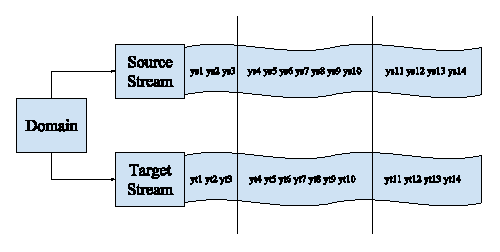
\includegraphics{fig_multistream.eps}
\caption{Demonstration of synchronous concept drift on data streams}
\label{fig:multistream}
\end{figure}

\section{Multistream Regression}
In this paper, we proposed a framework for multi-stream regression, referred as MSR. As we discussed before, in the multi-stream setting, the assumption of covariate shift holds valid between source and target streams until concept drift occurs in the target stream. Hence the objective of setting a MSR is to predict the output values in target stream efficiently using the information available in the source stream. To archive this goal, we establish two models. The first model is a regression model in the source stream with both input features and output values available. Parameters trained by this model can be used to make accurate prediction in source and target stream. We also applied a change detection technique (CDT) to detect concept drift in target stream. Once a concept drift is detected in the target stream, we will use the most recent data instances in the source stream to update the model, so that the covariate shift assumption can be restored. The flow chart of this algorithm is shown in Figure \ref{fig:flowchart}.

As shown in Figure \ref{fig:flowchart}, data instances in both 
source and target streams are generated continuously at the same time. The ensemble 
update is initialized by source and target streams, and training process starts on an initial mini-batch of data instances collected from head of source stream (Step 1 and 2). Then estimated output value of target stream is predicted via the trained model (Step 3).
Then, the generated predictions is used as an input for Drift Detection phase (Step 4). If a concept drift in target stream is detected by the algorithm, a new regression model is trained based on the latest minibatch data available in the source stream, so that bias in the stream can be removed (Step 6). The parameters of this ensemble model are further used for generating the output value of target stream.
\begin{figure}
\centering
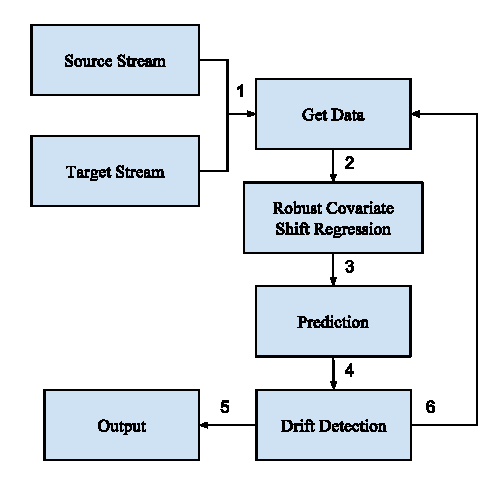
\includegraphics{fig_flowchart.eps}
\caption{Multistream Regression Overview}
\label{fig:flowchart}
\end{figure}

\makeatletter
\def\BState{\State\hskip-\ALG@thistlm}
\makeatother

\begin{algorithm}
\caption{Multistream Regression}\label{pse:MSR}
\begin{algorithmic}[1]
\Procedure{MSR}{}
\BState \textbf{begin}:
\State $B_s$, $B_t$ $\gets$ \textit{readData}$(S,T,I)$
\State $M \gets \textit{buildModel} (B_s, B_t)$
\While {$S$ or $T$ $exists$}
\State $B_s, B_t \gets readData(S,T,1)$
\State $W_s \gets getError(E_{param}, B_s)$
\State $W_t, \hat{Y} \gets preData(E_{param}, B_t)$
\If {$z \gets checkDrift(W_t)$}
\State $B_s, W_s \gets updateBuffer$$(z, B_s, W_s)$
\State $M \gets buildSourceModel(B_s)$
\EndIf
\State $\hat{y} \gets getPrediction(E_{param}, B_{t})$
\State print $getAccuracy (\hat{y}_t, B_t)$
\EndWhile
\EndProcedure
\end{algorithmic}
\end{algorithm}

\subsection{Initialization and Covariate Shift Correction}
In our proposed framework of MSR, data instances in source and target streams are stored in data buffer $B_s$ and $B_t$ respectively. Due to the nature of multi-stream regression setting, data in $B_s$ comes with output value, and data in $B_t$ arrives without output value. 

The RCSR algorithm is derived from minimax 
robust estimation \cite{chen}, which generates the predictor that minimizes the worst-case prediction loss. If the log loss function is employed as the loss 
function, this approach reduces to the principle of maximum entropy.
A natural loss function used to evaluate the conditional logloss on the target distribution is shown below:
\begin{equation}
\begin{split}
	\mathrm{reloss}_{f_{tgt}(\textbf{x})}(f(y|\textbf{\textbf{x}}), \hat{f}(y|\textbf{x}), f_0(y|\textbf{x})) \\
    = E_{f_{tgt}(\textbf{x})f(y|\textbf{x})}\left[-\mathrm{log}\frac{\hat{f}(y|\textbf{x})}{{f}_0(y|\textbf{x})}\right] % need change here
\end{split}
\end{equation}
Here, this conditional logloss evaluates the level of
covariate shift by measuring the ``surprise'' to tell samples from
$f_{tgt}(\textbf{x})f(y|\textbf{x})$ while actually is from $f_{tgt}(\textbf{x})\hat{f}
(y|\textbf{x})$ \cite{Lafferty01}.Thus, if there isn't significant 
covariate shift from the target set to the source set, the
solution could be a minimax robust estimation approach subjects to
quadratic squares solution for regression. Finally, the
regression estimator should be the one that is robust to data set that contains the most significant covariate shift. We define the difference in conditional logloss between an estimator $\hat{f}(y|\textbf{x})$ and a baseline condition distribution $f_0(y|\textbf{x})$ on the target stream distribution $f_{tgt}(x)f(y|\textbf{x})$ as relative loss in this equation.

Thus, the optimization problem of robust covariate shift regression can be interpreted as a two-player game in which the estimator first chooses $\hat{f}(y|\textbf{x})$ to minimize relative loss and then the adversarial evaluation player chooses $f(y|\textbf{x})$ to maximize relative loss. The estimator $\hat{f}(y|\textbf{x})$ is the saddle point solution of the following minimax optimization:
\begin{equation}
\begin{split}
	\mathrm{minimax} \; reloss_{f_{tgt}(\textbf{x})}(f(y|\textbf{x}), \hat{f}(y|\textbf{x}), f_0(y|\textbf{x}))
\end{split}
\end{equation}
Notice that the objective function of this optimization is convex and the constraints are each affine. Hence, standard tools from convex optimization can be deployed to obtain the solution for the constrained optimization.

The robust covariate shift regression for the target distribution $f_{tgt}(\textbf{x})$ predicted using constraints from the source distribution $f_{src}(\textbf{x})$ takes the form:
\begin{equation}
\begin{split}
	\hat{f}_{\theta}(y|x) = f_0(y|x)e^{-\frac{f_{src}(\textbf{x})}{f_{tgt}(\textbf{x})}\theta^T\Phi(\textbf{x},y)}
\end{split}
\end{equation}
\begin{equation}
\begin{split}
 	where: \; \Phi(\textbf{x},y) = \begin{bmatrix}
 y \\ 
 \textbf{x} \\1 
\end{bmatrix}
\begin{bmatrix}
  y&\textbf{x}&1 
\end{bmatrix}
\end{split}
\end{equation}
with parameters obtained via target distribution maximum conditional log likelihood estimation:
\begin{equation}\label{eqop}
\begin{split}
	\theta = \mathrm{arg} \, \mathrm{max}_{\theta} \, E_{f_{tgt}(\textbf{x})f(y|\textbf{x})}\left[\mathrm{log}\hat{f}_{\theta}(y|\textbf{x})\right]
\end{split}
\end{equation}
\begin{equation}
\begin{split}
	\theta^{T}vector(\Phi(\textbf{x},y)) =\begin{bmatrix}
 y \\ 
 \textbf{x} \\1 
\end{bmatrix}^T M
\begin{bmatrix}
y \\ 
 \textbf{x} \\1 
\end{bmatrix}
\end{split}
\end{equation}
Thus the robust covariate shift regression is a conditional Gaussian distribution:
\begin{equation}
\begin{split}
 	\hat{f}_M(y|\textbf{x}) \sim N(\mu(\textbf{x},M),\sigma^2(\textbf{x},M)) \\
    where: \; M = \begin{bmatrix}
 M_{(y,y)}&M_{(y,x_{1})} \\ 
 M_{(x_{1},y)}&M_{(1,1)} 
\end{bmatrix}
\end{split}
\end{equation}

\begin{equation} \label{eq1}
\begin{split}
\mu \left( \textbf{x}, M \right) = \left( 2\frac { f_{ src }\left( \textbf{x} \right)  }{ f_{ tgt }\left( \textbf{x} \right)  } M_{ (y,y) }+\frac { 1 }{ { \sigma  }^{ 2 } } { \mu  }_{ 0 } \right)^{-1} \\ 
  \left( -2\frac { f_{ src }\left( \textbf{x} \right)  }{ f_{ tgt }\left( \textbf{x} \right)  } M_{ y,x_{1} }\left[ \begin{matrix} \textbf{x} \\ 1 \end{matrix} \right] +\frac { 1 }{ { \sigma  }^{ 2 } } { \mu  }_{ 0 } \right)
\end{split}
\end{equation}

\subsection{Value Prediction}
Now we can use the matrix derived in Section \ref{challenges} to
predict value for every instance in the dataset. This
prediction is based on the Minimax estimation formulation, and
it minimizes the target distribution conditional
\emph{Kullback–Leibler} divergence. Hence the Covariate Shift problem
is addressed by this algorithm. Now the data in both source and target dataset are unbiased.


\subsection{Drift Detection}

In this section, a \emph{detectDrift} method is introduced to label those 
points in a data stream where significant changes happen. These changes are referred as concept drift.
We can use the generated $\hat{y}$ in the target set, along
with those instances with $y$ in the source set, to figure out 
the drift point in the target stream. 
A concept drift along $S$ could significantly impact the performance of
Multistream regression model. Here, the concept drift we mentioned
here specifically indicates a \emph{within-stream} drift. This type
of concept drift can cause change in the data distribution. Once
the change point is detected, the problem could be handled by
training another regression model so that the regression
parameters can be updated. We expect the prediction accuracy will be improved once we mark the drift points and update the regression model accordingly.

\subsubsection{Window Management}
In order to detect the change point accurately, two
sliding windows on both source stream and target stream are
maintained. The reason to do this is that we want to generate
feedback on most recent data.
The predicted value of data instances is generated by the
regression model, and is inserted into $W_t$. In the window,
there is an ensemble confidence score calculated from regression of data instances in $T$. Then values of confidence are generated 
within a range of [0,1]. Based on the nature of the confidence
level (confidence score value is usually low until there 
is a concept drift), here we apply a $beta$ distribution to model the
confidence level. Note that the window management schema for source 
stream is to follow the corresponding window in the target stream, so 
that most recent data can be used for training if there is a 
concept drift in the stream.

\subsubsection{Change Detection}
We propose a change point detection method to check for
significant change in the target stream. The reason of window management is to make the model check for concept drift, then update the prediction using most recent data automatically.

Algorithm 2 drafts our proposed CDT. If at any time point, the average feedback is below 0.5, or size of the the window exceeds $N_{max}$, the ensemble model is updated immediately regardless of any distribution change. Otherwise, this detection technique divides the window $W_h$ for each $q$ between $\gamma$ and $n-\gamma$, where $n$ is the total number of data instances and $\gamma$ is the cushion size. Thus, $W_h^b = W[1:q]$ is composed of older observations and $W_h^a=W[q+1:n]$ is composed of recent ones. Let $\theta_{a}$ and $\theta_{b}$ be the estimated distribution parameters from $W_h^a$ and $W_h^b$, we calculate the sum of log likelihood ratios as follows:

\begin{equation} \label{eq1}
\begin{split}
S\left ( q,n \right ) = \sum_{i=q+1}^{n}\textup{log}\left ( \frac{P(W_h[i] | \theta_{a}}{P(W_h[i] | \theta_{b}}  \right ) 
\end{split}
\end{equation}

where $P(W_h[i] | \theta)$ is the probability density function ,given a set of parameters $\theta$, applied on the $i^{th}$ instance stored in $W_h$. Using this output, $\omega_{n}$ can be calculated accordingly to determine whether a change point is detected.

\begin{algorithm}
\caption{Concept Drift Detection}\label{driftdetection}
\begin{algorithmic}[1]
\Procedure{detectDrift}{}
\BState \textbf{begin}:
\State \textit{Threshold} $\gets$ $-log({\alpha}_d)$, $n$ $\gets$ size of $W_h$, 
\State and $\omega_n$ $\gets$ 0
\If {$n \leq N_{max}$ $\&$ $mean(W_h[1:n] > 0.5$} 
\For {$q \gets \gamma$ : $n - \gamma$}
\State Estimate pre and post change distribution 
\State parameters, $\theta_{\alpha}$ and $\theta_{\beta}$ from $W_x[1:q]$ and 
\State $W_h[q+1:n]$ respectively
\State Calculate $S(q,n)$ using Equation (3)
\EndFor
\State $\omega_{n} = \max_{\gamma \leq q \leq n-\gamma}S(q,n)$
\If {$\omega_n \geq Threshold$}
\State \Return kmax, where $S_{kmax}=\omega_{n}$
\Else
\State \Return -1
\EndIf
\Else
\State \Return 0
\EndIf
\EndProcedure
\end{algorithmic}
\end{algorithm}
        

\subsection{Drift Adaption}
\label{driftadaption}
As we mentioned before, parameters generated by the regression
model will be updated once a concept drift is detected. If a drift is detected in the $T$ stream, new regressions are trained accordingly using a minibatch of recent data instances, which represents a new data distribution. However, the significance of each drift varies. Updates for each drift are not always necessary as it will increase the computational complexity dramatically. Here we assume that the covariate shift assumptions hold between the source and target stream initially. Since the drift occurs simultaneously on $S$ and $T$, for each detected drift in a stream, the associated data buffer ($B_s$ for $B_t$) and feedback buffer ($W_s$ or $W_t$) of the stream are updated by removing data instances before the change point, thereby simulating dynamic size of buffer. This is performed using $update$$Buffers$ in Algorithm \ref{pse:MSR}.


\section{Experiment}
\subsection{Datasets}
\subsubsection{Synthetic Dataset}
To evaluate the effectiveness of the algorithm, one way is to use synthetically generated data. Since normally there are two categories of concept drift, we generate our dataset based on the following two criteria, 1. local or global; 2. abrupt or gradual. 

For local concept drift, the data distribution changes only over a constrained region of instance space. On the other hand, for global concept drift, the distribution changes over the whole region of instance space, that is, for all the possible values in the target stream. Meanwhile, abrupt and gradual concept drift is the description of the sharpness of a specific drift. If the change happens suddenly and leads to a large drift within a short period, it can be referred as an abrupt drift. Otherwise, changes can be referred as a gradual drift.

Then, we start to simulate and study three scenarios for concept drift:

1. \emph{Global gradual drift}: The first type of simulated drift is global and gradual. The only occurrence of the gradual concept drift is at 1/2 of example of both source and target streams. Starting from this drift point, instances from the new concept are being gradually introduced among the examples to the old concept. 

2. \emph{Global abrupt drift}: The second type of simulated drift is global and abrupt. The concept drift appears over the whole instance space. There are one points of concept drift, which occurs at 1/2 of the example.

3. \emph{Local abrupt drift}: The third type of simulated drift is local and abrupt. Here, the concept drift appears in two distinct regions of the instance space. There are three points of abrupt change of both source and target streams, the first one at 1/4 of the examples, the second one at 1/2 of the examples, and the last one at 3/4 of the example.

\begin{table}[H]
\centering
\caption{Dataset}
\label{tab2}
\begin{tabular}{|l|l|l|}
\hline
 \bf{Dataset} & \bf{No. of features} & \bf{No. of instances} \\ \hline
 $globalGradual$ & 5 & 100,000\\ \hline
 $globalAbrupt$ & 5 & 100,000\\ \hline
 $localAbrupt$ & 5 & 100,000\\ \hline
 $bejingPM2.5$ & 12 & 43824 \\ \hline
 $bikeSharing$ & 16 & 17389 \\ \hline

\end{tabular}
\end{table}

\subsubsection{Real World Data}
We deploy publicly available regression datasets from the UCI repository \cite{liang2015}  to evaluate our approach. The number of instances and features can be found in Table 2 as well.

\begin{figure*} [h]
\centering
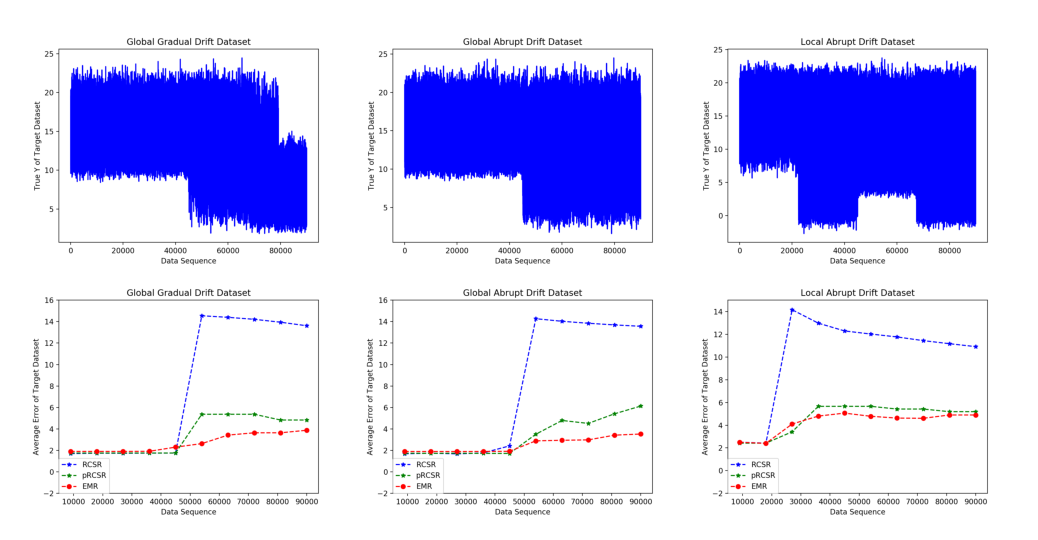
\includegraphics{fig_streamview_artificial.eps}
\caption{Stream: MAE on artificial datasets}
\label{fig:stream}
\end{figure*}

\begin{table*} [h]
\centering
\caption{Stream: MAE on artificial datasets}
\label{tab2}
\begin{tabular}{|l|l|l|l|l|l|l|l|l|l|}
\hline
          & \multicolumn{3}{l|}{globalAbrupt} & \multicolumn{3}{l|}{globalGradual} & \multicolumn{3}{l|}{localAbrupt} \\ \hline
Data Instance & RCSR       & pRCSR     & EMR      & RCSR       & pRCSR      & EMR      & RCSR      & pRCSR     & EMR      \\ \hline
9000       & \textbf{1.69}       & 1.74      & 1.90     & \textbf{1.71}       & 1.76       & 1.91     & 2.50      & \textbf{2.42}      & 2.50     \\ \hline
18000      & 1.75       & \textbf{1.73}      & 1.90     & \textbf{1.75}       & 1.76       & 1.91     & 2.42      & 2.42      & \textbf{2.40}     \\ \hline
27000      & \textbf{1.68}       & 1.74      & 1.90     & \textbf{1.74}       & 1.76       & 1.91     & 14.15     & \textbf{3.42}      & 4.10     \\ \hline
36000      & 1.77       & \textbf{1.73}      & 1.91     & \textbf{1.75}       & 1.76       & 1.92     & 12.97     & 5.66      & \textbf{4.80}     \\ \hline
45000      & 2.43       & \textbf{1.72}      & 1.92     & \textbf{1.76}       & 1.76       & 2.31     & 12.29     & 5.66      & \textbf{5.06}     \\ \hline
54000      & 14.27      & 3.51      & \textbf{2.89}     & 14.55      & 5.37       & \textbf{2.64}     & 12.02     & 5.66      & \textbf{4.78}     \\ \hline
63000      & 14.03      & 4.79      & \textbf{2.95}     & 14.40      & 5.37       & \textbf{3.43}     & 11.76     & 5.42      & \textbf{4.62}     \\ \hline
72000      & 13.85      & 4.52      & \textbf{2.98}     & 14.21      & 5.37       & \textbf{3.64}     & 11.43     & 5.42      & \textbf{4.66}     \\ \hline
81000      & 13.69      & 5.41      & \textbf{3.42}     & 13.94      & 4.83       & \textbf{3.94}     & 11.17     & 5.19      & \textbf{4.90}     \\ \hline
90000      & 13.56      & 6.13      & \textbf{3.53}     & 13.61      & 4.83       & \textbf{3.88}     & 10.91     & 5.19      & \textbf{4.90}     \\ \hline
\end{tabular}
\end{table*}


\subsection{Experiments}
\subsubsection{Baseline Method}

Since there aren't existing studies about regression problems under a
multistream setting, here we designed two baseline methods, including Robust Covariate Shift Regression 
(RCSR) and periodically update Robust Covariate Shift Regression (pRCSR). RCSR is the method described in Section
\ref{driftdetection} to eliminate the impact of covariate shift in between the source and target stream. And according to Chen's paper, the RCSR method has better performance on dataset with shift compared to normal method such as Multiple Linear Regression (MLR). Hence two baseline methods are designed as follows:



1. We follow the setting of RCSR to train 
regression parameters $M$. Just as the first baseline method, all the 
parameters are generated on an initial set of source and target data 
instances in both source and target stream. Then $M$ is used to predict 
all instances in $T$. Hence the difference between this baseline method 
and our proposed method in this paper is that this baseline method doesn't 
update the model based on the shift of probability density of data streams. We denote this baseline method as RCSR.

2. We update the RCSR model with periodically update. Generally speaking a new RCSR model is trained using the latest data instances in both $S$ and $T$ data streams. We assume the periodically update will improve the prediction accuracy of the model proposed. Here we denote this baseline method as pRCSR.


\subsection{Complexity Analysis}
At every iteration of MSR, a new data instance is obtained from both $S$ and $T$ streams. Hence the time complexity of this framework is highly depended on the regression we use. Since the prediction of output values is just a simple matrix multiplication, hence, the training process, which includes RCSR and drift detection, determines the complexity of the whole algorithm.

\begin{figure*} [h]
\centering
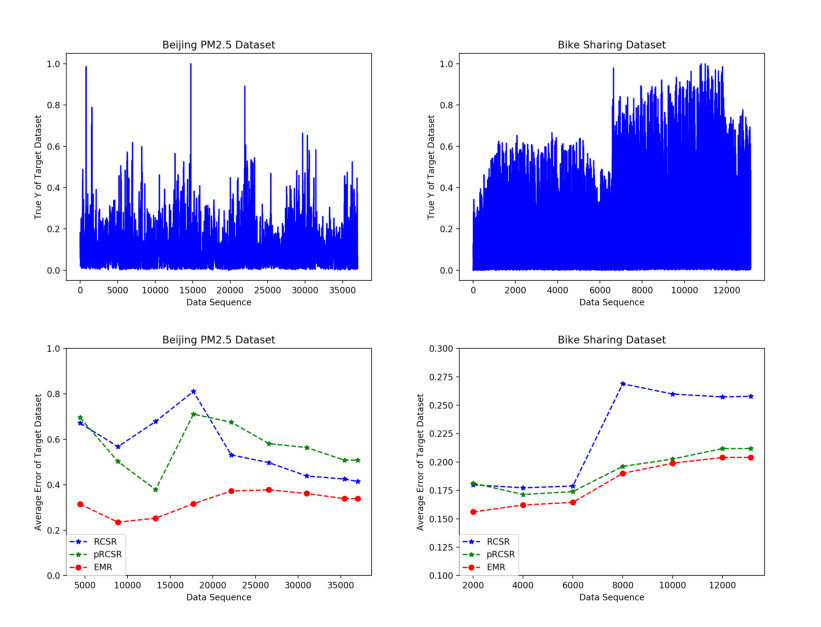
\includegraphics{fig_streamview_rel.eps}
\caption{Stream: MAE on real world datasets}
\label{fig:streamview_real}
\end{figure*}

\begin{table*}
\centering
\caption{Stream: MAE on real-world datasets}
\label{tab3}
\begin{tabular}{|l|l|l|l|l|l|l|l|}
\hline
              & \multicolumn{3}{l|}{Beijing PM2.5} &               & \multicolumn{3}{l|}{Bike Sharing} \\ \hline
Data Instance & RCSR   & pRCSR   & EMR             & Data Instance & RCSR   & pRSCR   & EMR            \\ \hline
4430          & 0.67   & 0.70    & \textbf{0.34}   & 2000          & 0.18   & 0.18    & \textbf{0.16}  \\ \hline
8860          & 0.57   & 0.50    & \textbf{0.23}   & 4000          & 0.18   & 0.17    & \textbf{0.16}  \\ \hline
13290         & 0.68   & 0.39    & \textbf{0.25}   & 6000          & 0.18   & 0.17    & \textbf{0.16}  \\ \hline
17720         & 0.81   & 0.71    & \textbf{0.32}   & 8000          & 0.27   & 0.20    & \textbf{0.20}  \\ \hline
22150         & 0.53   & 0.68    & \textbf{0.37}   & 10000         & 0.26   & 0.20    & \textbf{020}   \\ \hline
26580         & 0.50   & 0.58    & \textbf{0.38}            & 12000         & 0.26   & 0.21    & \textbf{0.20}  \\ \hline
31010         & 0.44   & 0.56    & \textbf{0.36}   & 13137         & 0/26   & 0.21    & \textbf{0.20}  \\ \hline
35440         & 0.42   & 0.51    & \textbf{0.34}   &               &        &         &                \\ \hline
37001         & 0.41   & 0.51    & \textbf{0.34}   &               &        &         &                \\ \hline
\end{tabular}
\end{table*}

RCSR is a minimax learning process trained by $B_s$. Since there isn't any training on the target stream, we can omit the time complexity on this part. With the time complexity of $O(n^2)$ for RCSR \cite{chen}, and the drift detection mechanism of $O(n^3)$ \cite{Haque1}. hence the overall time complexity of performing MSR is $O(n^3)$. 

\subsection{Results}

We evaluate the prediction accuracy using
Mean Absolute Error (MAE). Three approaches demonstrated in this figure are
our baseline approaches: RCSR and pRCSR approach, and our EMR approach. As shown in Figure 3 and 4, the progress of MAE is evaluated along with the target stream $T$. We can see that EMR has the smallest MAE compared to the other two baseline method once the concept drift occurs. Even though there are increasing of MAE along with the receiving of instances in the target stream, however the prediction accuracy of EMR still outperform both baseline method on all datasets by a significant margin, recovering from performance degradation, when necessary, using the drift detection mechanism. As we mentioned before, both baseline methods don't use any drift detection method. For instance, in the Global Abrupt Drift Dataset, all three methods share similar value of average errors until the abrupt drift occurs. The maximum MAE of EMR method on this dataset is 3.53, whereas results of RCSR and pRCSR are 13.56 and 6.13 accordingly.

According to these results, we also notice that the increasing trend of prediction error happens with the occurrence of concept drift simultaneously. The performance of RCSR, which is without any update along with the stream, is the worst among all three approaches. This result aligns with our expectation that model coefficients generated before the drift point is not representative to those data instances into the target stream after the drift point. Therefore, the prediction error of RCSR model is high after the drift point in all datasets. Meanwhile, the pRCSR model performs better than the RCSR due to the periodical updates. The updated coefficients is a significant improvement of prediction accuracy regarding the stream data. For example, in the Bike Sharing Dataset, the MAE of pRCSR stabilizes around 0.20 after the drift point, however, the RCSR reached to 0.26 by the end of 13,137 data instances in the target stream.


When comparing our proposed EMR approach with pRCSR, we can see that the prediction accuracy is even better. Our proposed EMR model consistently over perform the periodically updated RCSR proposal on every dataset. The reason is that even though pRCSR updates the model periodically, in most cases the update point won't match the drift point. That means there is a period between the drift point and periodical update point, predication is generated by old model coefficients. This fact will lead to an increasing MAE. On the other hand, due to the drift detection method applied in the model, which helps EMR to update the model coefficients once drift is detected, the regression model in EMR will be updated on a case-by-case basis. That means the regression model will only be updated when needed, and the time complexity is much less than update the model with higher frequency. Thus, the very existence of concept drift detection algorithm helps the RCSR model to get more accurate predictions in an efficient way.

% \begin{table}[H]
% \centering
% \caption{Stream: MAE on three datasets}
% \label{tab2}
% \begin{tabular}{|l|l|l|l|l|l|l|l|l|l|}
% \hline
%           & \multicolumn{3}{l|}{globalAbrupt} & \multicolumn{3}{l|}{globalGradual} & \multicolumn{3}{l|}{localAbrupt} \\ \hline
% Iteration & RCSR       & pRCSR     & EMR      & RCSR       & pRCSR      & EMR      & RCSR      & pRCSR     & EMR      \\ \hline
% 900       & 1.69       & 1.74      & 1.90     & 1.71       & 1.76       & 1.91     & 2.50      & 2.42      & 2.50     \\ \hline
% 1800      & 1.75       & 1.73      & 1.90     & 1.75       & 1.76       & 1.91     & 2.42      & 2.42      & 2.40     \\ \hline
% 2700      & 1.68       & 1.74      & 1.90     & 1.74       & 1.76       & 1.91     & 14.15     & 3.42      & 4.10     \\ \hline
% 3600      & 1.77       & 1.73      & 1.91     & 1.75       & 1.76       & 1.92     & 12.97     & 5.66      & 4.80     \\ \hline
% 4500      & 2.43       & 1.72      & 1.92     & 1.76       & 1.76       & 2.31     & 12.29     & 5.66      & 5.06     \\ \hline
% 5400      & 14.27      & 3.51      & 2.89     & 14.55      & 5.37       & 2.64     & 12.02     & 5.66      & 4.78     \\ \hline
% 6300      & 14.03      & 4.79      & 2.95     & 14.40      & 5.37       & 3.43     & 11.76     & 5.42      & 4.62     \\ \hline
% 7200      & 13.85      & 4.52      & 2.98     & 14.21      & 5.37       & 3.64     & 11.43     & 5.42      & 4.66     \\ \hline
% 8100      & 13.69      & 5.41      & 3.42     & 13.94      & 4.83       & 3.94     & 11.17     & 5.19      & 4.90     \\ \hline
% 9000      & 13.56      & 6.13      & 3.53     & 13.61      & 4.83       & 3.88     & 10.91     & 5.19      & 4.90     \\ \hline

% \end{tabular}
% \end{table}

\section{Conclusion and Future Work}
\label{conclusion}

In this paper, we propose an efficient multistream regression
framework to address the prediction problem in a multistream setting
Generally speaking, true value of dependent variable ($Y_s$) is only
available in the source stream, and is used to make
prediction for dependent variable of the target stream along with
independent variables of both streams ($X_s$ and $X_t$). 
Challenges of solving problems having covariate shift and
concept drift simultaneously in two data streams is widely
discussed. Our solution involves a minimax approach for
regression under covariate shift, and concept drift
detection techniques to correct drift. Following experiments
show that our solution has generated much better performance in
terms of MAE on various datasets, compared to baseline models.

There are some future work that we can think of to extend the use
of the proposed framework in this paper. For example, in this
paper we assume that concept drift happens
simultaneously in both source and target data stream. However,
concept drift can occur asynchronously as well. Hence there
are opportunities to discuss the effect of asynchronous drift on the prediction error as well.

%Appendix A

% \section{References}
% Generated by bibtex from your \texttt{.bib} file.  Run latex,
% then bibtex, then latex twice (to resolve references)
% to create the \texttt{.bbl} file.  Insert that \texttt{.bbl}
% file into the \texttt{.tex} source file and comment out
% the command \texttt{{\char'134}thebibliography}.
% % This next section command marks the start of
% % Appendix B, and does not continue the present hierarchy
% \section{More Help for the Hardy}

% Of course, reading the source code is always useful.  The file
% \path{acmart.pdf} contains both the user guide and the commented
% code.

% \begin{acks}
%   The authors would like to thank Dr. Yuhua Li for providing the
%   matlab code of  the \textit{BEPS} method. 

%   The authors would also like to thank the anonymous referees for
%   their valuable comments and helpful suggestions. The work is
%   supported by the \grantsponsor{GS501100001809}{National Natural
%     Science Foundation of
%     China}{http://dx.doi.org/10.13039/501100001809} under Grant
%   No.:~\grantnum{GS501100001809}{61273304}
%   and~\grantnum[http://www.nnsf.cn/youngscientsts]{GS501100001809}{Young
%     Scientsts' Support Program}.

% \end{acks}


% \section{Introduction}
% % no \IEEEPARstart
% This demo file is intended to serve as a ``starter file''
% for IEEE Computer Society conference papers produced under \LaTeX\ using
% IEEEtran.cls version 1.8b and later.
% % You must have at least 2 lines in the paragraph with the drop letter
% % (should never be an issue)
% I wish you the best of success.

% \hfill mds
 
% \hfill August 26, 2015

% \subsection{Subsection Heading Here}
% Subsection text here.


% \subsubsection{Subsubsection Heading Here}
% Subsubsection text here.


% % An example of a floating figure using the graphicx package.
% % Note that \label must occur AFTER (or within) \caption.
% % For figures, \caption should occur after the \includegraphics.
% % Note that IEEEtran v1.7 and later has special internal code that
% % is designed to preserve the operation of \label within \caption
% % even when the captionsoff option is in effect. However, because
% % of issues like this, it may be the safest practice to put all your
% % \label just after \caption rather than within \caption{}.
% %
% % Reminder: the "draftcls" or "draftclsnofoot", not "draft", class
% % option should be used if it is desired that the figures are to be
% % displayed while in draft mode.
% %
% %\begin{figure}[!t]
% %\centering
% %\includegraphics[width=2.5in]{myfigure}
% % where an .eps filename suffix will be assumed under latex, 
% % and a .pdf suffix will be assumed for pdflatex; or what has been declared
% % via \DeclareGraphicsExtensions.
% %\caption{Simulation results for the network.}
% %\label{fig_sim}
% %\end{figure}

% % Note that the IEEE typically puts floats only at the top, even when this
% % results in a large percentage of a column being occupied by floats.


% % An example of a double column floating figure using two subfigures.
% % (The subfig.sty package must be loaded for this to work.)
% % The subfigure \label commands are set within each subfloat command,
% % and the \label for the overall figure must come after \caption.
% % \hfil is used as a separator to get equal spacing.
% % Watch out that the combined width of all the subfigures on a 
% % line do not exceed the text width or a line break will occur.
% %
% %\begin{figure*}[!t]
% %\centering
% %\subfloat[Case I]{\includegraphics[width=2.5in]{box}%
% %\label{fig_first_case}}
% %\hfil
% %\subfloat[Case II]{\includegraphics[width=2.5in]{box}%
% %\label{fig_second_case}}
% %\caption{Simulation results for the network.}
% %\label{fig_sim}
% %\end{figure*}
% %
% % Note that often IEEE papers with subfigures do not employ subfigure
% % captions (using the optional argument to \subfloat[]), but instead will
% % reference/describe all of them (a), (b), etc., within the main caption.
% % Be aware that for subfig.sty to generate the (a), (b), etc., subfigure
% % labels, the optional argument to \subfloat must be present. If a
% % subcaption is not desired, just leave its contents blank,
% % e.g., \subfloat[].


% % An example of a floating table. Note that, for IEEE style tables, the
% % \caption command should come BEFORE the table and, given that table
% % captions serve much like titles, are usually capitalized except for words
% % such as a, an, and, as, at, but, by, for, in, nor, of, on, or, the, to
% % and up, which are usually not capitalized unless they are the first or
% % last word of the caption. Table text will default to \footnotesize as
% % the IEEE normally uses this smaller font for tables.
% % The \label must come after \caption as always.
% %
% %\begin{table}[!t]
% %% increase table row spacing, adjust to taste
% %\renewcommand{\arraystretch}{1.3}
% % if using array.sty, it might be a good idea to tweak the value of
% % \extrarowheight as needed to properly center the text within the cells
% %\caption{An Example of a Table}
% %\label{table_example}
% %\centering
% %% Some packages, such as MDW tools, offer better commands for making tables
% %% than the plain LaTeX2e tabular which is used here.
% %\begin{tabular}{|c||c|}
% %\hline
% %One & Two\\
% %\hline
% %Three & Four\\
% %\hline
% %\end{tabular}
% %\end{table}


% % Note that the IEEE does not put floats in the very first column
% % - or typically anywhere on the first page for that matter. Also,
% % in-text middle ("here") positioning is typically not used, but it
% % is allowed and encouraged for Computer Society conferences (but
% % not Computer Society journals). Most IEEE journals/conferences use
% % top floats exclusively. 
% % Note that, LaTeX2e, unlike IEEE journals/conferences, places
% % footnotes above bottom floats. This can be corrected via the
% % \fnbelowfloat command of the stfloats package.




% \section{Conclusion}
% The conclusion goes here.




% % conference papers do not normally have an appendix



% % use section* for acknowledgment
% \ifCLASSOPTIONcompsoc
%   % The Computer Society usually uses the plural form
%   \section*{Acknowledgments}
% \else
%   % regular IEEE prefers the singular form
%   \section*{Acknowledgment}
% \fi


% The authors would like to thank...





% trigger a \newpage just before the given reference
% number - used to balance the columns on the last page
% adjust value as needed - may need to be readjusted if
% the document is modified later
%\IEEEtriggeratref{8}
% The "triggered" command can be changed if desired:
%\IEEEtriggercmd{\enlargethispage{-5in}}

% references section

% can use a bibliography generated by BibTeX as a .bbl file
% BibTeX documentation can be easily obtained at:
% http://mirror.ctan.org/biblio/bibtex/contrib/doc/
% The IEEEtran BibTeX style support page is at:
% http://www.michaelshell.org/tex/ieeetran/bibtex/
%\bibliographystyle{IEEEtran}
% argument is your BibTeX string definitions and bibliography database(s)
%\bibliography{IEEEabrv,../bib/paper}
%
% <OR> manually copy in the resultant .bbl file
% set second argument of \begin to the number of references
% (used to reserve space for the reference number labels box)


% \begin{thebibliography}{1}

% \bibitem{IEEEhowto:kopka}
% H.~Kopka and P.~W. Daly, \emph{A Guide to \LaTeX}, 3rd~ed.\hskip 1em plus
%   0.5em minus 0.4em\relax Harlow, England: Addison-Wesley, 1999.

% \end{thebibliography}


\bibliographystyle{IEEEref}
\bibliography{sigproc} 



% that's all folks
\end{document}


